\section{Diagrama de Definição de Bloco}

\subsubsection{O que é diagrama de definição de blocos}

O diagrama de definições de bloco é baseado no diagrama de classes da UML com o adicional de algumas restrições e extensões definidas dentro da SysML. Sendo o diagrama mais usado dentro dessa. Sua função é modelar os aspectos estruturais, através de blocos, de um sistema, mostrando os elementos físicos, relacionamentos, fluxos e hierarquias.

\subsubsection{Estrutura dos diagramas de definição de blocos}

Com a proposta de mostrar diferentes elementos do fluxo e suas relações a figura abaixo mostra o diagrama de definição de blocos de uma ACME câmera, com os símbolos mais comuns do diagrama de blocos.

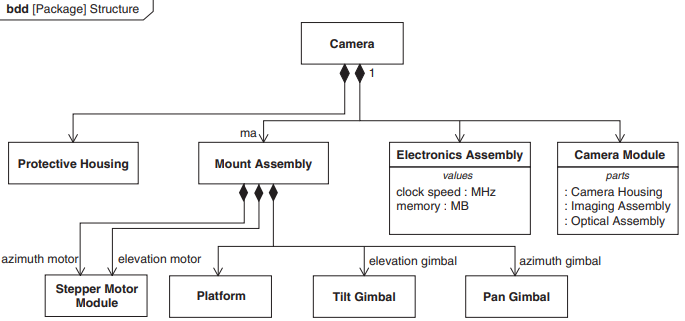
\includegraphics[width=\textwidth,height=\textheight,keepaspectratio]{figures/diagrama de blocos.PNG}

\paragraph{}
 \textbf{Elementos físicos} 
 
 
Os elementos físicos são graficamente representados por blocos. Eles podem ser hardwares, softwares, pessoas ou qualquer outra entidade lógica ou conceitual. 

O nome do bloco aparece em seu topo em negrito, enquanto as outras propriedades tem seus compartimentos abaixo em letra minúscula, itálico e espaço entre as palavras. Essas propriedades podem ser de três diferentes tipos. 

Uma delas é propriedade de parte, que decompõem o bloco nos elementos que os constituem, por exemplo, no diagrama acima, dentro do bloco de "Camera Module"  tem-se as partes "Camera Housing", "Imaging Assembly"  e "Optical Assembly".

Outra é a propriedade de referência, que referencia partes de outro bloco indicando em que partes o blocos conectados se relacionam. 

Por fim, pode-se ter também a propriedade de valor, responsável por descrever as características quantificáveis do bloco, no diagrama acima, o bloco "Eletronics Assembly"  tem as propriedades de valor "clock speed"  em MHz e "memory"  em MB.

\paragraph{}
 \textbf{Relacionamento entre blocos} 
 
O relacionamento entre blocos indica como os blocos se relacionam, de maneira geral ele é representado com uma linha simples com elementos nas pontas, que irá indicar qual a relação exata entre eles. Existem quatro tipos diferentes de relação que podem ser representados no diagrama de blocos.

A conexão de composição é representada graficamente por um losango preenchido conectado em um bloco maior com um traço embaixo ligando a outros blocos, é utilizado para indicar que o bloco maior possui outros elementos definindo assim uma propriedade de parte no bloco maior. Existe a possibilidade de se colocar uma seta na outra parte, neste caso faz alusão a alguma propriedade referência. A propriedade de parte é escrita no diagrama em cima do bloco de chegada quando o nome do bloco em si não oferece informações suficientes, enquanto a propriedade de referência é escrita em cima do bloco de partida. No diagrama acima, o bloco "Mount Assembly", por exemplo esta ligado desta maneira aos blocos "Stepper Motor Module" duas vezes, em relação as partes "azimuth motor" e ao "elevation motor", já na relação entre o bloco "Camera" e "Eletronics Assembly" não foi necessário indicar o nome da parte de referência, uma vez que o próprio bloco descreve bem o ponto de conexão.

A conexão de referência é representada graficamente por um losangolo vazio em uma ponta ligado por uma seta a outros elementos. Ela é utilizada para indicar que um bloco referencia o outro, quando existe uma referencia apenas de um lado da relação é utilizada uma seta no bloco que contém a propriedade de referência, já se ambos blocos se referenciam entre si não são utilizadas setas. As referencias, quando não indicadas como propriedades do bloco, são escritas em cima do bloco, da mesma maneira que as propriedades de parte na conexão de composição. 

A conexão por associação 